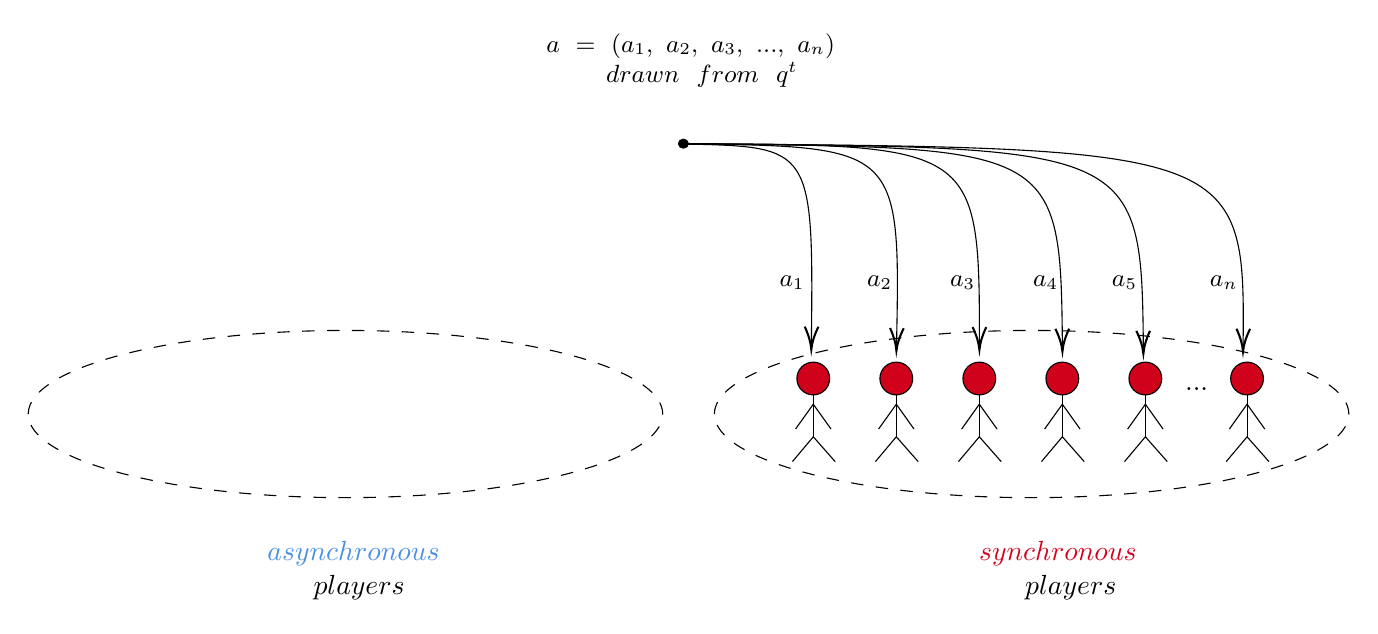
\begin{tikzpicture}[x=0.75pt,y=0.75pt,yscale=-1,xscale=1]
%uncomment if require: \path (0,341); %set diagram left start at 0, and has height of 341

%Shape: Ellipse [id:dp3005583251278674] 
\draw  [dash pattern={on 4.5pt off 4.5pt}] (13.72,205.29) .. controls (13.72,183.04) and (82.16,165) .. (166.57,165) .. controls (250.99,165) and (319.42,183.04) .. (319.42,205.29) .. controls (319.42,227.53) and (250.99,245.57) .. (166.57,245.57) .. controls (82.16,245.57) and (13.72,227.53) .. (13.72,205.29) -- cycle ;
%Shape: Ellipse [id:dp8969793505161732] 
\draw  [dash pattern={on 4.5pt off 4.5pt}] (344.3,205.29) .. controls (344.3,183.04) and (412.74,165) .. (497.15,165) .. controls (581.57,165) and (650,183.04) .. (650,205.29) .. controls (650,227.53) and (581.57,245.57) .. (497.15,245.57) .. controls (412.74,245.57) and (344.3,227.53) .. (344.3,205.29) -- cycle ;
%Curve Lines [id:da2811571509974371] 
\draw    (329.37,75.01) .. controls (433.58,76.55) and (434.1,75.93) .. (432.03,173.35) ;
\draw [shift={(432,174.82)}, rotate = 271.22] [color={rgb, 255:red, 0; green, 0; blue, 0 }  ][line width=0.75]    (10.93,-3.29) .. controls (6.95,-1.4) and (3.31,-0.3) .. (0,0) .. controls (3.31,0.3) and (6.95,1.4) .. (10.93,3.29)   ;
%Curve Lines [id:da7257100915393806] 
\draw    (329.37,75.01) .. controls (471.39,75.56) and (472.1,75.56) .. (472,172.86) ;
\draw [shift={(472,174.33)}, rotate = 270.06] [color={rgb, 255:red, 0; green, 0; blue, 0 }  ][line width=0.75]    (10.93,-3.29) .. controls (6.95,-1.4) and (3.31,-0.3) .. (0,0) .. controls (3.31,0.3) and (6.95,1.4) .. (10.93,3.29)   ;
%Curve Lines [id:da9281274979524605] 
\draw    (329.37,75.17) .. controls (510.2,76.56) and (511.1,75.93) .. (511.99,173.66) ;
\draw [shift={(512,175.14)}, rotate = 269.48] [color={rgb, 255:red, 0; green, 0; blue, 0 }  ][line width=0.75]    (10.93,-3.29) .. controls (6.95,-1.4) and (3.31,-0.3) .. (0,0) .. controls (3.31,0.3) and (6.95,1.4) .. (10.93,3.29)   ;
%Shape: Ellipse [id:dp5747949043348641] 
\draw  [fill={rgb, 255:red, 0; green, 0; blue, 0 }  ,fill opacity=1 ] (327,75.01) .. controls (327,73.82) and (328.06,72.85) .. (329.37,72.85) .. controls (330.69,72.85) and (331.75,73.82) .. (331.75,75.01) .. controls (331.75,76.21) and (330.69,77.17) .. (329.37,77.17) .. controls (328.06,77.17) and (327,76.21) .. (327,75.01) -- cycle ;
%Shape: Ellipse [id:dp9839795244213729] 
\draw  [fill={rgb, 255:red, 208; green, 2; blue, 27 }  ,fill opacity=1 ] (424.06,188.17) .. controls (424.06,183.8) and (427.59,180.27) .. (431.96,180.27) .. controls (436.32,180.27) and (439.85,183.8) .. (439.85,188.17) .. controls (439.85,192.53) and (436.32,196.06) .. (431.96,196.06) .. controls (427.59,196.06) and (424.06,192.53) .. (424.06,188.17) -- cycle ;
%Straight Lines [id:da42311535821122725] 
\draw    (431.96,196.06) -- (431.96,216.62) ;
%Straight Lines [id:da6182167576414703] 
\draw    (431.96,216.24) -- (421.91,228.2) ;
%Straight Lines [id:da3414399202354139] 
\draw    (431.96,216.24) -- (442.5,228.2) ;
%Straight Lines [id:da8812076043056545] 
\draw    (431.96,200.55) -- (423.42,212.51) ;
%Straight Lines [id:da24598080293534452] 
\draw    (431.96,200.55) -- (440.49,212.51) ;
%Shape: Ellipse [id:dp42077037172884646] 
\draw  [fill={rgb, 255:red, 208; green, 2; blue, 27 }  ,fill opacity=1 ] (464.06,188.17) .. controls (464.06,183.8) and (467.59,180.27) .. (471.96,180.27) .. controls (476.32,180.27) and (479.85,183.8) .. (479.85,188.17) .. controls (479.85,192.53) and (476.32,196.06) .. (471.96,196.06) .. controls (467.59,196.06) and (464.06,192.53) .. (464.06,188.17) -- cycle ;
%Straight Lines [id:da4649866978988264] 
\draw    (471.96,196.06) -- (471.96,216.62) ;
%Straight Lines [id:da20370020373133868] 
\draw    (471.96,216.24) -- (461.91,228.2) ;
%Straight Lines [id:da6428389436293447] 
\draw    (471.96,216.24) -- (482.5,228.2) ;
%Straight Lines [id:da026158760314009655] 
\draw    (471.96,200.55) -- (463.42,212.51) ;
%Straight Lines [id:da012714818764540947] 
\draw    (471.96,200.55) -- (480.49,212.51) ;
%Shape: Ellipse [id:dp9386780214229125] 
\draw  [fill={rgb, 255:red, 208; green, 2; blue, 27 }  ,fill opacity=1 ] (384.06,188.17) .. controls (384.06,183.8) and (387.59,180.27) .. (391.96,180.27) .. controls (396.32,180.27) and (399.85,183.8) .. (399.85,188.17) .. controls (399.85,192.53) and (396.32,196.06) .. (391.96,196.06) .. controls (387.59,196.06) and (384.06,192.53) .. (384.06,188.17) -- cycle ;
%Straight Lines [id:da8416342905135632] 
\draw    (391.96,196.06) -- (391.96,216.62) ;
%Straight Lines [id:da971411093876879] 
\draw    (391.96,216.24) -- (381.91,228.2) ;
%Straight Lines [id:da25510054563755324] 
\draw    (391.96,216.24) -- (402.5,228.2) ;
%Straight Lines [id:da5957049019216363] 
\draw    (391.96,200.55) -- (383.42,212.51) ;
%Straight Lines [id:da7516626238989643] 
\draw    (391.96,200.55) -- (400.49,212.51) ;
%Shape: Ellipse [id:dp31349873946910845] 
\draw  [fill={rgb, 255:red, 208; green, 2; blue, 27 }  ,fill opacity=1 ] (504.06,188.17) .. controls (504.06,183.8) and (507.59,180.27) .. (511.96,180.27) .. controls (516.32,180.27) and (519.85,183.8) .. (519.85,188.17) .. controls (519.85,192.53) and (516.32,196.06) .. (511.96,196.06) .. controls (507.59,196.06) and (504.06,192.53) .. (504.06,188.17) -- cycle ;
%Straight Lines [id:da9274690734516102] 
\draw    (511.96,196.06) -- (511.96,216.62) ;
%Straight Lines [id:da009461491957432733] 
\draw    (511.96,216.24) -- (501.91,228.2) ;
%Straight Lines [id:da7157941275449011] 
\draw    (511.96,216.24) -- (522.5,228.2) ;
%Straight Lines [id:da10712131031014893] 
\draw    (511.96,200.55) -- (503.42,212.51) ;
%Straight Lines [id:da7164052851513101] 
\draw    (511.96,200.55) -- (520.49,212.51) ;
%Shape: Ellipse [id:dp7955315984240003] 
\draw  [fill={rgb, 255:red, 208; green, 2; blue, 27 }  ,fill opacity=1 ] (544.06,188.17) .. controls (544.06,183.8) and (547.59,180.27) .. (551.96,180.27) .. controls (556.32,180.27) and (559.85,183.8) .. (559.85,188.17) .. controls (559.85,192.53) and (556.32,196.06) .. (551.96,196.06) .. controls (547.59,196.06) and (544.06,192.53) .. (544.06,188.17) -- cycle ;
%Straight Lines [id:da6098435626058583] 
\draw    (551.96,196.06) -- (551.96,216.62) ;
%Straight Lines [id:da5218065763701105] 
\draw    (551.96,216.24) -- (541.91,228.2) ;
%Straight Lines [id:da5919508403198068] 
\draw    (551.96,216.24) -- (562.5,228.2) ;
%Straight Lines [id:da34102824578192137] 
\draw    (551.96,200.55) -- (543.42,212.51) ;
%Straight Lines [id:da12215875066269422] 
\draw    (551.96,200.55) -- (560.49,212.51) ;
%Shape: Ellipse [id:dp8836820382228234] 
\draw  [fill={rgb, 255:red, 208; green, 2; blue, 27 }  ,fill opacity=1 ] (593.06,188.17) .. controls (593.06,183.8) and (596.59,180.27) .. (600.96,180.27) .. controls (605.32,180.27) and (608.85,183.8) .. (608.85,188.17) .. controls (608.85,192.53) and (605.32,196.06) .. (600.96,196.06) .. controls (596.59,196.06) and (593.06,192.53) .. (593.06,188.17) -- cycle ;
%Straight Lines [id:da9730808708372152] 
\draw    (600.96,196.06) -- (600.96,216.62) ;
%Straight Lines [id:da5119326823281014] 
\draw    (600.96,216.24) -- (590.91,228.2) ;
%Straight Lines [id:da013412651363815753] 
\draw    (600.96,216.24) -- (611.5,228.2) ;
%Straight Lines [id:da0010693670034451763] 
\draw    (600.96,200.55) -- (592.42,212.51) ;
%Straight Lines [id:da3253282682883363] 
\draw    (600.96,200.55) -- (609.49,212.51) ;
%Curve Lines [id:da12457767898807792] 
\draw    (329.37,75.17) .. controls (549,76.56) and (550.1,75.93) .. (550.99,174.64) ;
\draw [shift={(551,176.14)}, rotate = 269.49] [color={rgb, 255:red, 0; green, 0; blue, 0 }  ][line width=0.75]    (10.93,-3.29) .. controls (6.95,-1.4) and (3.31,-0.3) .. (0,0) .. controls (3.31,0.3) and (6.95,1.4) .. (10.93,3.29)   ;
%Curve Lines [id:da24506091904522598] 
\draw    (329.37,75.17) .. controls (598.75,76.56) and (600.1,78.54) .. (599.02,173.7) ;
\draw [shift={(599,175.14)}, rotate = 270.66] [color={rgb, 255:red, 0; green, 0; blue, 0 }  ][line width=0.75]    (10.93,-3.29) .. controls (6.95,-1.4) and (3.31,-0.3) .. (0,0) .. controls (3.31,0.3) and (6.95,1.4) .. (10.93,3.29)   ;
%Curve Lines [id:da5780300577298003] 
\draw    (329.37,75.17) .. controls (391.79,76.56) and (392.1,75.93) .. (391.02,172.67) ;
\draw [shift={(391,174.14)}, rotate = 270.64] [color={rgb, 255:red, 0; green, 0; blue, 0 }  ][line width=0.75]    (10.93,-3.29) .. controls (6.95,-1.4) and (3.31,-0.3) .. (0,0) .. controls (3.31,0.3) and (6.95,1.4) .. (10.93,3.29)   ;

% Text Node
\draw (121.03,263.61) node [anchor=north west][inner sep=0.75pt]    {$ \begin{array}{l}
\textcolor[rgb]{0.29,0.56,0.89}{asynchronous}\\
\ \ \ \ \ players
\end{array}$};
% Text Node
\draw (463.91,263.61) node [anchor=north west][inner sep=0.75pt]    {$ \begin{array}{l}
\textcolor[rgb]{0.82,0.01,0.11}{synchronous}\\
\ \ \ \ \ players
\end{array}$};
% Text Node
\draw (569.83,191.37) node [anchor=north west][inner sep=0.75pt]    {$...$};
% Text Node
\draw (374.49,137.4) node [anchor=north west][inner sep=0.75pt]  [font=\small]  {$a_{1}$};
% Text Node
\draw (416.59,137.4) node [anchor=north west][inner sep=0.75pt]  [font=\small]  {$a_{2}$};
% Text Node
\draw (581.83,137.4) node [anchor=north west][inner sep=0.75pt]  [font=\small]  {$a_{n}$};
% Text Node
\draw (255.42,19.4) node [anchor=north west][inner sep=0.75pt]  [font=\small]  {$ \begin{array}{l}
\bm{a}\ =\ ( a_{1} ,\ a_{2} ,\ a_{3} ,\ ...,\ a_{n})\\
\ \ \ \ \ \ \ drawn\ \ from\ \ \bm{q}^t
\end{array}$};
% Text Node
\draw (456.59,137.4) node [anchor=north west][inner sep=0.75pt]  [font=\small]  {$a_{3}$};
% Text Node
\draw (496.59,137.4) node [anchor=north west][inner sep=0.75pt]  [font=\small]  {$a_{4}$};
% Text Node
\draw (534.59,137.4) node [anchor=north west][inner sep=0.75pt]  [font=\small]  {$a_{5}$};


\end{tikzpicture}
